\documentclass{article}
\usepackage{microtype,graphicx,booktabs}
\usepackage{balance}
\usepackage{hyperref}
\usepackage[preprint]{icml2026}
\usepackage{amsmath,amssymb,amsthm,mathtools}
\usepackage{tikz}
\usetikzlibrary{arrows.meta,calc,angles,quotes}
\usepackage[capitalize,noabbrev]{cleveref}
\newtheorem{theorem}{Theorem}[section]
\newtheorem{proposition}[theorem]{Proposition}
\theoremstyle{definition}
\newtheorem{definition}[theorem]{Definition}
\newtheorem{hypothesis}[theorem]{Hypothesis}
\DeclareMathOperator{\Var}{Var}
\DeclareMathOperator{\tr}{tr}
\DeclareMathOperator{\Rea}{Re}
\DeclareMathOperator{\Imma}{Im}
\DeclareMathOperator{\polar}{polar}
\newcommand{\E}{\mathbb E}
\newcommand{\R}{\mathbb R}
\newcommand{\C}{\mathbb C}
\newcommand{\Id}{\mathsf I}
\newcommand{\T}{\mathsf T}
\newcommand{\G}{\mathsf G}
\newcommand{\Q}{\mathsf Q}
\newcommand{\Proj}{\mathsf P}
\newcommand{\M}{\mathsf M}
\newcommand{\U}{\mathsf U}
\newcommand{\Stretch}{\mathsf S}
\newcommand{\Hol}{\mathsf H}
\newcommand{\J}{\mathsf J}
\newcommand{\Rot}{\mathsf R}
\newcommand{\norm}[1]{\left\lVert#1\right\rVert}
\newcommand{\ip}[2]{\left\langle#1,#2\right\rangle}
\definecolor{routeblue}{HTML}{0072B2}
\definecolor{routeorange}{HTML}{D55E00}
\renewcommand{\today}{November 2, 2026}
\icmltitlerunning{An Information-Theoretic Principle of Prediction: Synchronicity}
\hypersetup{pdftitle={An Information-Theoretic Principle of Prediction: Synchronicity},pdfauthor={Zhenyu Li}}
\begin{document}
\twocolumn[
\icmltitle{\texorpdfstring{An Information-Theoretic Principle of Prediction:\\Synchronicity}{An Information-Theoretic Principle of Prediction: Synchronicity}}
\begin{icmlauthorlist}
\icmlauthor{Zhenyu Li}{zju}
\end{icmlauthorlist}
\icmlaffiliation{zju}{Zhejiang University}
\icmlcorrespondingauthor{Zhenyu Li}{zylics@zju.edu.cn}
\icmlkeywords{Prediction, information theory, synchronicity, complex information, geometric phase}
\vskip 0.3in
]
\printAffiliationsAndNotice{}
\begin{abstract}
Prediction is possible when a present record constrains the future continuations of a process. We formulate synchronicity as the shared relational organization through which records, intermediate responses, and later outcomes obey such constraints. A conditional-prediction operator gives a unified description of information amount, recoverable future distinctions, and their transport between response contexts. Complex information records the magnitude and orientation of paired predictive distinctions; information phase measures their relative orientation after alternative routes of interpretation and response. A rhombic propagation--recombination geometry connects these definitions to exact prediction-error identities, a quarter-turn example, and the acquisition of useful information from residual error. We also propose an informationon construction in which complex relational amplitudes generate Lorentzian interval geometry and a phase connection, providing a concrete physical hypothesis for the same organization.
\end{abstract}
\section{Prediction as a Shared Relation}
\label{sec:prediction}
A shepherd places one stone in a bag for each sheep that enters an enclosure. Before counting the sheep again, the shepherd can use the stones to predict the result. The present stones and the later count refer to the same organized process: a one-to-one registration was made, the registration persisted, and changes to the flock were either prevented or recorded. The example makes prediction concrete. Something available now constrains an outcome that has not yet been read.

Similar organization supports a neural network's forecast, an animal's anticipation, and a machine's coordinated action. Information passes through several forms: a physical relation, a record, a transformation of that record, and a response. Some relations remain distributed among components. Their consequences can be collected through several routes, whose agreement depends on how the components preserve and compare the relevant distinctions. We call this shared organization \emph{synchronicity}.

The statistical foundation is classical information theory. Shannon information measures how records reduce uncertainty about selected alternatives~\citep{shannon1948}. Conditional-expectation geometry resolves which functions of those alternatives are recoverable~\citep{calmon2017}; usable-information theory makes the reader's computational resources explicit~\citep{xu2020}. Our concern is the ordered organization of those recoverable distinctions: how they spread through parallel responses, are compared, and return as a prediction or action.

The geometry in \cref{fig:diamond} is central to this account. An initiating event and a later readout delimit a region of possible propagation. Intermediate responses can coexist across a spatial cut, while each route has an order. Recombination brings those routes back to a common question. The unresolved interior represents continuations that share the available boundary records. Prediction consists of identifying what these continuations already have in common. Phase describes how a distinction changes orientation when carried through their response structure.

\begin{figure*}[t]
\centering
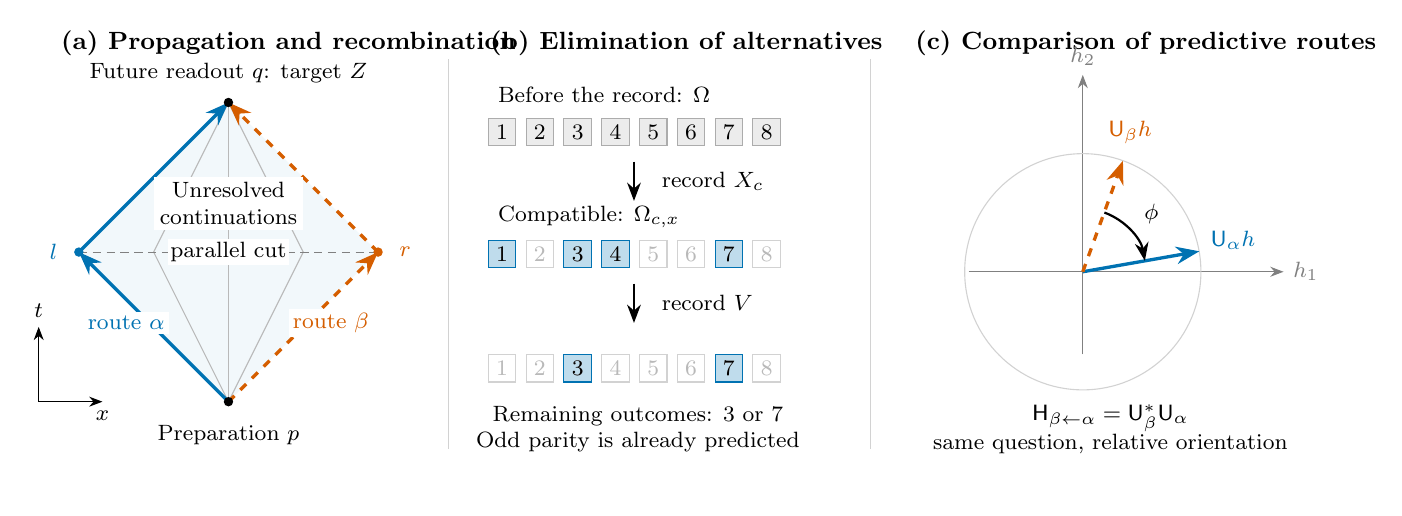
\begin{tikzpicture}[x=1cm,y=1cm,>=Stealth,font=\footnotesize]
\path[use as bounding box] (-.3,-.5) rectangle (16.8,5.35);
\node[anchor=west,font=\bfseries\small] at (0,5.15) {(a) Propagation and recombination};
\fill[routeblue!5] (2.25,.6)--(.35,2.5)--(2.25,4.4)--(4.15,2.5)--cycle;
\draw[gray!55,thin] (2.25,.6)--(1.3,2.5)--(2.25,4.4);
\draw[gray!55,thin] (2.25,.6)--(3.2,2.5)--(2.25,4.4);
\draw[gray!55,thin] (2.25,.6)--(2.25,4.4);
\draw[routeblue,very thick,->] (2.25,.6)--(.35,2.5);
\draw[routeblue,very thick,->] (.35,2.5)--(2.25,4.4);
\draw[routeorange,very thick,dashed,->] (2.25,.6)--(4.15,2.5);
\draw[routeorange,very thick,dashed,->] (4.15,2.5)--(2.25,4.4);
\draw[gray,densely dashed] (.35,2.5)--(4.15,2.5);
\fill (2.25,.6) circle (1.7pt);
\fill (2.25,4.4) circle (1.7pt);
\fill[routeblue] (.35,2.5) circle (1.7pt);
\fill[routeorange] (4.15,2.5) circle (1.7pt);
\node[anchor=north,align=center] at (2.25,.42) {Preparation $p$};
\node[anchor=south,align=center] at (2.25,4.53) {Future readout $q$: target $Z$};
\node[routeblue,anchor=east] at (.2,2.5) {$l$};
\node[routeorange,anchor=west] at (4.3,2.5) {$r$};
\node[routeblue,fill=white,inner sep=1.5pt] at (.95,1.6) {route $\alpha$};
\node[routeorange,fill=white,inner sep=1.5pt] at (3.55,1.6) {route $\beta$};
\node[fill=white,inner sep=2pt,align=center] at (2.25,3.12) {Unresolved\\continuations};
\node[fill=white,inner sep=1pt] at (2.25,2.5) {parallel cut};
\draw[->,thin] (-.16,.6)--(-.16,1.55) node[above] {$t$};
\draw[->,thin] (-.16,.6)--(.65,.6) node[below] {$x$};

\draw[gray!35] (5.05,0)--(5.05,4.95);
\node[anchor=west,font=\bfseries\small] at (5.45,5.15) {(b) Elimination of alternatives};
\node[anchor=west] at (5.55,4.5) {Before the record: $\Omega$};
\foreach \k in {0,...,7}{\draw[fill=gray!15,draw=gray!65] (5.55+.48*\k,3.85) rectangle +(0.35,.35);}
\foreach \k in {0,...,7}{\pgfmathtruncatemacro{\outcome}{\k+1}\node at (5.725+.48*\k,4.025) {\outcome};}
\draw[->,thick] (7.4,3.65)--(7.4,3.15);
\node[anchor=west] at (7.63,3.4) {record $X_c$};
\node[anchor=west] at (5.55,2.95) {Compatible: $\Omega_{c,x}$};
\foreach \k in {0,...,7}{\draw[fill=white,draw=gray!35] (5.55+.48*\k,2.3) rectangle +(0.35,.35);}
\foreach \k in {0,2,3,6}{\draw[fill=routeblue!25,draw=routeblue] (5.55+.48*\k,2.3) rectangle +(0.35,.35);}
\foreach \k in {0,...,7}{\pgfmathtruncatemacro{\outcome}{\k+1}\node[text=gray!55] at (5.725+.48*\k,2.475) {\outcome};}
\foreach \k in {0,2,3,6}{\pgfmathtruncatemacro{\outcome}{\k+1}\node at (5.725+.48*\k,2.475) {\outcome};}
\draw[->,thick] (7.4,2.1)--(7.4,1.6);
\node[anchor=west] at (7.63,1.85) {record $V$};
\foreach \k in {0,...,7}{\draw[fill=white,draw=gray!35] (5.55+.48*\k,.85) rectangle +(0.35,.35);}
\foreach \k in {2,6}{\draw[fill=routeblue!25,draw=routeblue] (5.55+.48*\k,.85) rectangle +(0.35,.35);}
\foreach \k in {0,...,7}{\pgfmathtruncatemacro{\outcome}{\k+1}\node[text=gray!55] at (5.725+.48*\k,1.025) {\outcome};}
\foreach \k in {2,6}{\pgfmathtruncatemacro{\outcome}{\k+1}\node at (5.725+.48*\k,1.025) {\outcome};}
\node[align=center] at (7.45,.25) {Remaining outcomes: $3$ or $7$\\Odd parity is already predicted};

\draw[gray!35] (10.4,0)--(10.4,4.95);
\node[anchor=west,font=\bfseries\small] at (10.85,5.15) {(c) Comparison of predictive routes};
\begin{scope}[yshift=.4cm]
\draw[->,gray] (11.65,1.85)--(15.65,1.85) node[right] {$h_1$};
\draw[->,gray] (13.1,.8)--(13.1,4.35) node[above] {$h_2$};
\draw[gray!35] (13.1,1.85) circle (1.5);
\draw[routeblue,very thick,->] (13.1,1.85)--(14.58,2.11);
\draw[routeorange,very thick,dashed,->] (13.1,1.85)--(13.61,3.26);
\node[routeblue,anchor=west] at (14.6,2.25) {$\U_\alpha h$};
\node[routeorange,anchor=south] at (13.7,3.35) {$\U_\beta h$};
\draw[->,thick] (13.374,2.602) arc[start angle=70,end angle=10,radius=.8];
\node at (13.97,2.58) {$\phi$};
\end{scope}
\node[align=center] at (13.45,.25) {$\Hol_{\beta\leftarrow\alpha}=\U_\beta^*\U_\alpha$\\same question, relative orientation};
\end{tikzpicture}

\caption{Prediction joins distributed evidence to a common future question. \textbf{(a)} A causal diamond joins preparation \(p\) to future readout \(q\); two forward routes \(\alpha,\beta\) sample and combine intermediate responses, while the shaded interior contains unresolved continuations. \textbf{(b)} Records restrict the candidate outcomes to 3 and 7, determining odd parity before the outcome is read. \textbf{(c)} Registering the same predictive distinction along two routes gives a relative transformation \(\Hol_{\beta\leftarrow\alpha}=\U_\beta^*\U_\alpha\); its angle is information phase. The spacetime sketch uses \(c=1\).}
\label{fig:diamond}
\end{figure*}

We develop one mathematical object throughout: a family of conditional-prediction operators together with registration maps between their recoverable modes. Its norm measures predictive strength, its polar factors separate changes of strength from changes of orientation, and comparisons of alternative routes give information phase. The construction makes the meaning of the complex plane explicit: its coordinates are paired future distinctions, and its angle determines which combination a response addresses.

The paper first states the prediction principle and its Shannon specialization (\cref{sec:information}). It then defines complex information and phase within the rhombic geometry, and derives observable prediction-error consequences (\cref{sec:phase,sec:consequences}). Learning appears as the acquisition and reuse of further predictive relations (\cref{sec:learning}). Finally, a spinorial informationon hypothesis gives a common algebraic construction of causal intervals and phase transport (\cref{sec:informationons}). Proofs and calibration procedures are collected in the appendices.



\section{The Information-Theoretic Principle}
\label{sec:information}
\subsection{Records and admissible continuations}
Let \((\Omega,\mu)\) describe admissible realizations of a process. A realization includes both the available records and the later outcome. Write \(Z:\Omega\to\mathcal Z\) for a future target, \(\nu\) for its distribution, and \(X_c:\Omega\to\mathcal X_c\) for the record available in context \(c\). A context specifies which observations and response operations are available. The initial development uses finite alphabets and \(\nu(z)>0\); square-integrable continuous examples are considered below.

Observing \(X_c=x\) restricts the process to the compatible continuations
\begin{equation}
\begin{aligned}
\Omega_{c,x}&=\{\omega:X_c(\omega)=x\},\\
p_c(z\mid x)&=\mu(Z=z\mid X_c=x).
\end{aligned}
\label{eq:posterior}
\end{equation}
For noisy measurements, likelihood weights perform the same restriction probabilistically. Zero likelihood removes a continuation; unequal likelihoods change its weight. The target event is specified before its outcome is read. The conditional law can be calibrated from previous realizations or derived from a model of the process.

\begin{definition}[Predictive synchronicity]
A present record and a future distinction have predictive synchronicity when they share a reproducible constraint in the joint process law. For a centered future contrast \(h(Z)\), its strength in context \(c\) is
\begin{equation}
\mathcal S_c(h)=\Var\!\left(\E[h(Z)\mid X_c]\right).
\label{eq:synchronicity}
\end{equation}
\end{definition}
This definition gives the term a specific role: it measures the part of a future contrast that varies systematically with the present record. Multiple records can supply a joint constraint even when each alone is uninformative. For independent fair bits \(A,B\) and target \(Z=A\oplus B\), either bit leaves one bit of uncertainty, while their pair determines \(Z\).

In \cref{fig:diamond}(b), the records leave \(Z\in\{3,7\}\). The future outcome remains variable, while its odd parity is already fixed. Prediction can determine a property before resolving the entire event.

\begin{theorem}[Prediction principle]
\label{thm:prediction}
For any square-integrable centered contrast \(h(Z)\), the optimal prediction from \(X_c\) is \(\widehat h_c=\E[h(Z)\mid X_c]\), and
\begin{equation}
\min_g\E[(h(Z)-g(X_c))^2]
=\norm h_\nu^2-\mathcal S_c(h).
\label{eq:prediction}
\end{equation}
The contrast is determined by the record exactly when it is constant, up to conditional null sets, on each compatible continuation class \(\Omega_{c,x}\).
\end{theorem}
The result is the conditional-expectation projection theorem, here used as the organizing principle of prediction. Under logarithmic loss, the corresponding reduction in optimal expected loss is \(I(Z;X_c)\). Thus classical information amount and contrast-specific predictive strength describe the same joint relation at different resolutions.

For the sheep count, write the later number as \(Z=X+\Delta\), where \(X\) is the registered count and \(\Delta\) accounts for subsequent arrivals, departures, births, or losses. The prediction is \(X+\E[\Delta\mid X]\). Recording \(\Delta\) or ensuring \(\Delta=0\) makes the count exact. Stable registration and a law for intervening changes are the physical content supporting the inference. Finite counters and continuous mechanical systems both realize such continuation constraints.

\subsection{One operator for amount and structure}
Let \(\mathcal H=L_0^2(\nu)\) be the space of centered future contrasts, with \(\ip{h}{k}_\nu=\E[h(Z)k(Z)]\). Define
\begin{equation}
\boxed{\T_c h=\E[h(Z)\mid X_c],\qquad
\G_c=\T_c^*\T_c.}
\label{eq:operator}
\end{equation}
Then \(\mathcal S_c(h)=\ip{h}{\G_ch}_\nu\), with \(0\preceq\G_c\preceq\Id\). Eigenvectors of \(\G_c\) identify future questions recoverable from the record; eigenvalues give their predictive strengths. This is the conditional-estimation geometry underlying principal inertia components~\citep{calmon2017}.

The units are fixed by a binary discrimination experiment. Let a fair calibration bit \(B\) select \(\nu_b(z)=\nu(z)[1+b\epsilon h(z)]\), with \(|\epsilon|\norm h_\infty<1\), while the response channel \(p(X_c\mid Z)\) is held fixed. Then
\begin{equation}
I(B;X_c)=\frac{\epsilon^2}{2\ln2}\ip{h}{\G_ch}_\nu+O(\epsilon^4)
\quad\text{bits}.
\label{eq:calibration}
\end{equation}
This experiment calibrates the strength of a distinction through response statistics. Ordinary forecasts evaluate \(\T_ch\) on the record currently available.

For a family \(\mathcal O\) of available operations on retained state \(R\), define the information potential of a contrast by
\begin{equation*}
\mathcal P_{\mathcal O}(h)=\sup_{o\in\mathcal O}
\norm{\E[h(Z)\mid X_o]}^2.
\end{equation*}
When \(Z\to R\to X_o\), this is bounded by \(\norm{\E[h(Z)\mid R]}^2\). If the present readout belongs to \(\mathcal O\), the difference \(\mathcal P_{\mathcal O}(h)-\mathcal S_c(h)\) is available but unused predictive strength. Source-dependent new observations enter the accounting as additional evidence.

\subsection{The common mathematical form}
The full predictive description consists of \((\Omega,\mu,Z,\{X_c\},\{\M_{dc}\})\), where \(\M_{dc}\) registers predictive modes between contexts. Its calculation follows one chain:
\begin{equation}
\begin{gathered}
p_c(z\mid x)\ \longrightarrow\ \T_c\ \longrightarrow\ \G_c,\\
\M_{dc}=\U_{dc}\Stretch_{dc},\qquad
\Hol_{\beta\leftarrow\alpha}=\U_\beta^*\U_\alpha.
\end{gathered}
\label{eq:spine}
\end{equation}
The first line measures prediction. The second measures how its distinctions are registered, stretched, and compared across routes. \Cref{sec:phase} specifies these maps and gives the complex plane its operational meaning.

\section{Complex Information and the Rhombic Structure}
\label{sec:phase}
\subsection{What a complex informational coordinate means}
Consider two orthonormal future contrasts \(h_1,h_2\). They might ask whether an object will move left or right and whether it will move up or down. Their span is a plane of possible predictive questions. A distinction \(h=a h_1+b h_2\) has the complex coordinate
\begin{equation}
\boxed{\psi(h)=a+ib,\qquad
\J h_1=h_2,\quad\J h_2=-h_1.}
\label{eq:complex}
\end{equation}
We call \(\psi\) a \emph{complex information amplitude}. Its magnitude specifies the size of the contrast; its argument specifies which combination of future alternatives it distinguishes. The plane carries the statistical metric inherited from \(\mathcal H\), and its orientation fixes the sign of the argument.

A response aligned with \(h_1\) addresses the real component. A response aligned with \(h_2\) addresses its quadrature companion. A change in response organization can make the second component available where the first was previously read. At angle \(\pi\), the same distinction is read with reversed sign; at \(\pi/2\), the response addresses the orthogonal question. These meanings are determined by the calibrated questions and response, so a phase describes an informational relation rather than a media label.

The Shannon calibration follows from \cref{eq:calibration}. For \(\G_c=\lambda\Id\) on this plane, the leading information is \(\epsilon^2\lambda|\psi|^2/(2\ln2)\) bits. For an arbitrary \(\G_c\), the same amount is the quadratic form \(\epsilon^2\ip{h}{\G_ch}/(2\ln2)\). Thus the statistical metric supplies the scale, while the complex coordinate retains orientation.

\begin{proposition}[Composition in the complex plane]
\label{prop:complex}
An oriented real two-mode map \(\M\) acts by scalar complex multiplication exactly when \(\M\J=\J\M\). In compatible orthonormal frames,
\begin{equation*}
\M=\begin{pmatrix}a&-b\\b&a\end{pmatrix}
\quad\Longrightarrow\quad\psi'=(a+ib)\psi.
\end{equation*}
For a general real two-mode map, \(\psi'=\kappa_+\psi+\kappa_-\overline\psi\), with \(\kappa_+,\kappa_-\) given in \cref{app:proofs}.
\end{proposition}
This gives complex information an operation law. In the scalar case, consecutive responses multiply amplitudes and add phases. The two-coefficient form also represents reflection and unequal gains along the two predictive directions.

\subsection{Parallel extent and ordered depth}
The rhombus in \cref{fig:diamond} has a direct spacetime realization. For an initiating event \(p\) and later readout event \(q\), the causal diamond is
\begin{equation}
\mathcal D(p,q)=J^+(p)\cap J^-(q).
\label{eq:diamond}
\end{equation}
The future of \(p\) describes where its effects can reach; the past of \(q\) describes which effects can contribute to that readout. Their intersection expands and then contracts across intermediate spatial cuts. In flat \(1+1\)-dimensional spacetime, with \(p=(0,0)\), \(q=(T,0)\), and \(c=1\), the allowed slice is \(|x|\le\min(t,T-t)\).

The informational counterpart is a region of compatible continuations. Intermediate variables are summed out when computing an endpoint response, while their joint constraints remain in the resulting conditional law. This gives the ``bubble'' its meaning: its interior contains unresolved realization detail, and its boundary carries the conditions used to compare possible outcomes. Spatial extent represents parallel participation; depth represents ordered composition. A future readout event specifies the question whose answer will be obtained, while the answer itself remains the target \(Z\).

In null coordinates \(u=t+x\), \(v=t-x\), reciprocal rescaling
\begin{equation}
u'=e^\chi u,\qquad v'=e^{-\chi}v,
\qquad du'\,dv'=du\,dv
\label{eq:squeeze}
\end{equation}
preserves the interval while changing the coordinate balance between the two directions. This is a precise form of mutual stretching and compression. The physical conjecture in \cref{sec:informationons} places it in the same complex matrix representation as rotations and phase transport.

\subsection{Registration of predictive questions}
Choose a rank-\(r\) spectral band of \(\G_c\), separated by a gap from the other modes. Let \(\Proj_c\) be its projector and \(\Q_c\) an orthonormal frame in the common space \(\mathcal H\). The entries of a coefficient vector now refer to explicit future contrasts.

Transferring a predictive distinction from context \(c\) to context \(d\) by least-squares matching gives the registration map
\begin{equation}
\M_{dc}=\Q_d^*\Q_c=\U_{dc}\Stretch_{dc},
\quad
\Stretch_{dc}=(\M_{dc}^*\M_{dc})^{1/2}.
\label{eq:registration}
\end{equation}
For nonsingular overlap, \(\U_{dc}=\polar(\M_{dc})\) is unique. The positive factor measures overlap strengths; the orthogonal factor preserves the comparison of directions. Equivalently, \(\U_{dc}\) minimizes \(\norm{\Q_dU-\Q_c}_F\) over orthogonal \(U\). This is a concrete registration operation on predictions.

A system's implemented registration can also be measured by presenting calibrated probes and regressing its transferred coefficients in the endpoint frame. In that case \(\M_{dc}\) denotes the measured transfer, and the same polar decomposition separates gain from orientation. The measurement protocol records which registration is used. Smooth least-squares registration obeys the projector transport equation
\begin{equation*}
\dot h=[\dot\Proj,\Proj]h,
\qquad h\in\operatorname{Ran}\Proj,
\end{equation*}
the standard minimum-change transport of subspaces~\citep{bendokat2023}.

\begin{definition}[Information phase]
\label{def:phase}
Let \(\alpha\) and \(\beta\) be two registered routes between the same contexts, with ordered orientation products \(\U_\alpha\) and \(\U_\beta\). Their relative information transport and phase spectrum are
\begin{equation}
\boxed{\Hol_{\beta\leftarrow\alpha}=\U_\beta^*\U_\alpha,
\qquad\operatorname{spec}(\Hol)=\{e^{i\phi_k}\}.}
\label{eq:phase}
\end{equation}
On an oriented real two-mode sector with \(\Hol\in SO(2)\), the information phase is the angle \(\phi\) in \(\Hol=\Rot(\phi)\), modulo \(2\pi\).
\end{definition}

Information phase is therefore the relative orientation of a predictive distinction after its response routes are compared. A zero phase means the two registrations align that distinction; a nonzero phase tells how to rotate one registration to match the other. Comparing a route with a fixed reference is the open-path case. Returning to the initial context gives the closed-loop case, or holonomy. The return is a comparison in predictive-question space; the physical process can continue forward throughout.

Changing local frames \(\Q_c\mapsto\Q_cV_c\) conjugates \(\Hol\) at the starting context, preserving its eigenphases. A signed planar angle uses an oriented frame; reflection reverses that convention. For smooth geometric transport, the ordered route determines the phase independently of its traversal speed. This is the geometric-phase structure developed by Pancharatnam, Berry and Simon~\citep{pancharatnam1956,berry1984,simon1983}, here applied to statistically calibrated predictive distinctions.

\section{What Phase Predicts}
\label{sec:consequences}
\subsection{A quarter-turn with unchanged information amount}
Let the future target vector be \(Z\sim\mathcal N(0,\Id_3)\). In context \(n\), the available record is
\begin{equation*}
X_n=A_nZ+\eta,\qquad \eta\sim\mathcal N(0,\sigma^2\Id_2),
\end{equation*}
where \(A_n\) has orthonormal rows perpendicular to a unit normal \(n\), and \(\sigma>0\). This joint law calibrates a forecast from \(X_n\) to \(Z\). It has an equivalent prospective realization: first draw \(X_n\sim\mathcal N(0,(1+\sigma^2)\Id_2)\), then draw the later target from its Gaussian conditional law, given in \cref{app:example}.

On linear future contrasts \(h_v(Z)=v^TZ\),
\begin{equation}
\G_n=\frac{I-nn^T}{1+\sigma^2},\qquad
I(Z;X_n)=\log_2(1+\sigma^{-2}).
\label{eq:example}
\end{equation}
Both predictive strengths in the observable plane stay fixed as \(n\) changes. Register the modes along the short great-circle arcs \(e_z\to e_x\to e_y\to e_z\). Initial questions \((e_x,e_y)\) return as \((e_y,-e_x)\), giving
\begin{equation*}
\Hol=\begin{pmatrix}0&-1\\1&0\end{pmatrix},\qquad\phi=\pi/2.
\end{equation*}
The current record has the same total mutual information and the same observable plane at the endpoint. The first tracked question now predicts the second target component. A weak shift of the first target component produces a different response, and inverse registration restores the original prediction. Phase identifies this change in what the response means.

\subsection{A predictive penalty for misregistration}
The statistical consequence can be quantified for two-mode predictive readouts. Let \(w\in\R^2\) be a calibrated record with \(\E w=0\) and \(\E[ww^T]=\Id_2/2\). Suppose the future target has conditional law \(\mathcal N(K_*w,\sigma^2\Id_2)\), and a predictor reports \(\mathcal N(Kw,\sigma^2\Id_2)\).

\begin{proposition}[Amplitude and phase in predictive loss]
\label{prop:loss}
The excess expected log loss in nats is
\begin{equation}
\mathcal R=\frac{\norm{K-K_*}_F^2}{4\sigma^2}.
\label{eq:loss}
\end{equation}
For \(K=a\Rot(\phi)\) and \(K_*=b\Rot(\phi_*)\), with \(a,b\ge0\),
\begin{equation}
\mathcal R=\frac{a^2+b^2-2ab\cos(\phi-\phi_*)}{2\sigma^2}.
\label{eq:phaseloss}
\end{equation}
\end{proposition}
Thus equally strong responses can have different forecasting performance because they address differently oriented target distinctions. The predictor and target are compared in the same calibrated coordinates. A geometric route supplies \(K\) when its implemented links realize the stated registration; measured links supply it directly.

\subsection{Estimating the predictive structure}
For finite alphabets, the matrix
\begin{equation*}
B_c(x,z)=\frac{\sqrt{\nu(z)}\,p(X_c=x\mid Z=z)}{\sqrt{p_c(x)}}
\end{equation*}
represents \(\T_c\) in whitened coordinates. Restricting \(B_c^*B_c\) to the subspace orthogonal to \(\sqrt\nu\) gives \(\G_c\). A finite dictionary of future contrasts and record features provides a regression-based approximation for larger systems. The calibration records can come from completed episodes; a deployed forecast uses its current record and the resulting predictive operator.

Estimate \(\G_c\), choose a stable band, register neighboring frames, and compute the relative route product in \cref{eq:phase}. Report predictive strengths together with phase. Spectral gaps control subspace sensitivity~\citep{yu2015}, while the smallest singular value of neighboring overlaps controls registration sensitivity. For orthogonal links with aligned errors \(\norm{\widehat\U_j-\U_j}\le\delta_j\),
\begin{equation*}
\norm{\widehat\Hol-\Hol}\le\sum_j\delta_j.
\end{equation*}
For planar rotations, a bound \(\delta\le2\) gives principal angular error at most \(2\arcsin(\delta/2)\). \Cref{app:errors} also gives an error bound for actual transfer products and a resulting interval for predictive loss. These calculations reduce a calibrated family of responses to mode strengths and route comparisons.

\section{Residuals, Learning, and Reusable Prediction}
\label{sec:learning}
The unexplained part of an outcome is relative to the available record. For a future contrast \(h(Z)\), let
\begin{equation*}
r_c=h(Z)-\T_ch(X_c).
\end{equation*}
When an additional record \(V\) becomes available, its contribution is the part of this residual that it predicts:
\begin{equation}
\Delta_c=\E[r_c\mid X_c,V],\qquad
\widehat h_{c,V}=\widehat h_c+\Delta_c.
\label{eq:residual}
\end{equation}
Orthogonality of conditional expectation gives the exact improvement
\begin{equation}
\E[r_c^2]-\E[(r_c-\Delta_c)^2]=\E[\Delta_c^2].
\label{eq:improvement}
\end{equation}
For logarithmic loss the corresponding improvement is \(I(Z;V\mid X_c)\). The useful part of new evidence is therefore its relation to what remains unresolved. A record with considerable variability can contribute little when it repeats an already available distinction.

This interpretation clarifies elimination. For noise-free records, successive observations intersect compatible continuation classes. For noisy records, they revise the weights of those classes. Their expected predictive benefit is given by \cref{eq:improvement} or conditional mutual information. A particular observation can expose more uncertainty than expected; the conditional law records that change as part of the same process.

Learning retains a reusable approximation to these relations. It can improve the conditional predictor \(\T_c\), make additional modes of \(\G_c\) accessible, or improve the registrations \(\M_{dc}\) that let different components work with the same distinctions. The resulting memory may be located in model parameters, a physical configuration, an external record, or their joint relation. This connects predictive-state approaches~\citep{shalizi2001} with the computational accessibility emphasized by usable information~\citep{xu2020}.

The rhombus organizes this activity without requiring a fixed number of stages. Responses open several routes; evidence restricts their possible continuations; comparison aligns what those routes imply; and recombination leaves a reusable prediction. The earlier a--d intuition can be read as a coarse description of this circulation. A measured phase gives an angular comparison of selected predictive modes within it.

For a retained summary \(R=f(H)\) of history \(H\), the ideal log-loss advantage of the full history under a controlled probe \(A\) is \(I(H;Z\mid R,A)\). A system that detects such a gap has evidence that its present representation omits a predictive distinction. Seeking a record that explains the residual is then a concrete route from detected incompleteness to further learning. The same construction applies when other agents or the surrounding environment retain the missing relation.

\section{An Informationon Construction}
\label{sec:informationons}
\subsection{From relational amplitudes to event geometry}
The preceding theory describes prediction through records and responses. We now propose a physical realization in which elementary relational amplitudes generate both event geometry and comparison phase. The construction uses the spinor representation of Lorentzian geometry~\citep{penrose1960}. Information-space approaches based on elementary process events have also been explored by \citet{sulis2014}; the elementary object used here is specified by the following hypothesis.

\begin{hypothesis}[Informationon realization]
An informationon is an elementary realization event carrying a two-component complex amplitude \(\xi\in\C^2\), together with relations specifying its admissible predecessors. Its projected event increment is
\begin{equation}
\boxed{\delta\mathsf x=\ell\xi\xi^\dagger,
\qquad \mathsf x=x^0\Id+\sum_{k=1}^3x^k\sigma_k,}
\label{eq:infoon}
\end{equation}
where \(\sigma_k\) are the Pauli matrices and \(\ell>0\) fixes the physical realization scale. Event coordinates accumulate these increments along admissible routes; routes meeting at a common event obey the corresponding sum-consistency condition.
\end{hypothesis}

Here the two entries of \(\xi\) may be viewed as a pair of complex informational modes. They carry internal relational coordinates before a spacetime position is assigned. Their quadratic projection has real four-component coordinates and satisfies
\begin{equation}
\det\mathsf x=(x^0)^2-\sum_{k=1}^3(x^k)^2.
\label{eq:interval}
\end{equation}
A single increment has \(\det\delta\mathsf x=0\) and \(\delta x^0\ge0\). Sums of non-collinear increments are future timelike. Thus a positive ordering of elementary realizations projects to a causal cone, and two common endpoints delimit the rhombic region of \cref{eq:diamond}.

For example, the two rank-one increments \(\ell|0\rangle\langle0|\) and \(\ell|1\rangle\langle1|\) add to \(\ell\Id\). The increments \(\ell|+\rangle\langle+|\) and \(\ell|-\rangle\langle-|\) have the same sum. Different intermediate realizations can therefore agree on an endpoint event. A coarse record can retain that endpoint relation while leaving the intermediate route unresolved.

A general construction generates such agreement directly. Collect \(m\) amplitudes into \(\Psi=(\xi_1,\ldots,\xi_m)\). For any unitary \(V\in U(m)\), the columns of \(\Psi V\) give a different elementary decomposition with the same completion:
\begin{equation}
\boxed{\mathsf x_q-\mathsf x_p=\ell\Psi\Psi^\dagger
=\ell(\Psi V)(\Psi V)^\dagger.}
\label{eq:completion}
\end{equation}
Successive column sums describe a future-directed route. Choosing \(V\) randomly changes the intermediate route while preserving the completion. A present record of an invariant of \(\Psi\Psi^\dagger\) therefore predicts that part of the endpoint before the route is realized. This is an explicit model of the prediction principle based on a shared constraint.

This realizes the LED-banner intuition: an extended pattern is a relation among elementary updates and their projections. Pattern continuity is carried by that relation, while successive realizations supply its local support. An intrinsic realization label orders the updates used in a description; observable interval and phase comparisons are expressed through their relations.

\subsection{Compression and rotation in one complex frame law}
For \(A\in SL(2,\C)\), the transformation
\begin{equation*}
\xi\mapsto A\xi,\qquad
\mathsf x\mapsto A\mathsf xA^\dagger
\end{equation*}
preserves \(\det\mathsf x\) and the future cone. A particularly informative family is
\begin{equation}
A(\chi,\vartheta)=
\begin{pmatrix}
e^{(\chi+i\vartheta)/2}&0\\
0&e^{-(\chi+i\vartheta)/2}
\end{pmatrix}.
\label{eq:complexframe}
\end{equation}
Writing \(u=x^0+x^3\), \(v=x^0-x^3\), and \(w=x^1-ix^2\), it gives
\begin{equation}
u'=e^\chi u,\qquad v'=e^{-\chi}v,
\qquad w'=e^{i\vartheta}w.
\label{eq:uv}
\end{equation}
The real parameter produces reciprocal stretching of null directions; the imaginary parameter rotates a transverse relation. Both preserve the same determinant \(uv-|w|^2\). Hyperbolic compression and compact rotation thus have a common complex matrix representation, with distinct transformation parameters.

For a collection of informationons the two actions combine as \(\Psi\mapsto A\Psi V\). The left action transforms the interval coordinates, while the right action changes the unresolved decomposition at fixed completion. The amplitude-factor geometry \(\rho=WW^\dagger\) and its comparison transport have an established formulation in Uhlmann's work~\citep{uhlmann1986}. Here that structure is assigned the role of organizing elementary event realizations.

The relation to prediction is structural. A present record specifies part of the joint realization, and the admissible increments and endpoint conditions restrict its continuations. The rhombic organization supplies a way to compare distributed partial realizations with a common future event. The informational calculation remains the conditional law in \cref{eq:posterior}; \cref{eq:infoon} proposes a physical origin for the organization on which that calculation depends.

\subsection{An internal phase and its connection}
The projection \(\xi\xi^\dagger\) is unchanged by \(\xi\mapsto e^{i\theta}\xi\). Normalizing \(n=\xi/\norm\xi\), comparisons between nonorthogonal representatives give
\begin{equation}
\mathcal U_{dc}=\frac{n_d^\dagger n_c}{|n_d^\dagger n_c|},
\qquad
e^{i\Phi_\gamma}=\prod_{(c,d)\in\gamma}\mathcal U_{dc}.
\label{eq:spinphase}
\end{equation}
Local changes of representative multiply a link by endpoint phases that cancel around the loop. This is the rank-one complex version of the registration law in \cref{eq:phase}. For a smooth coarse field \(n(x)\), its connection is \(\mathcal A_\mu=-i n^\dagger\partial_\mu n\), with curvature \(\mathcal F_{\mu\nu}=\partial_\mu\mathcal A_\nu-\partial_\nu\mathcal A_\mu\). The loop phase is \(-\oint\mathcal A\) in this convention. The projected event geometry and the internal phase connection therefore arise from the same amplitude representation.

This connection gives an explicit nonzero phase. For
\begin{equation*}
n_0=(1,0)^T,\quad
n_1=(1,1)^T/\sqrt2,\quad
n_2=(1,i)^T/\sqrt2,
\end{equation*}
the loop \(n_0\to n_1\to n_2\to n_0\) has \(\Phi=-\pi/4\). The internal relation returns while sums of positive event increments continue to advance. Relational recurrence and forward physical progress coexist in this construction.

Random fluctuations can be introduced covariantly. One explicit conditional ensemble is \(\xi\sim\mathcal{CN}(0,\mathsf C)\), with \(\mathsf C\succ0\). It has \(\E[\delta\mathsf x]=\ell\mathsf C\), and transforms consistently under \((\xi,\mathsf C)\mapsto(A\xi,A\mathsf CA^\dagger)\). The covariance describes local physical conditions. A full physical dynamics specifies how these conditions and the weights of compatible event graphs evolve. The informationon hypothesis places those dynamical choices on a common representation of intervals, fluctuations, and phase; the explicit construction above establishes their algebraic compatibility.

\section{Relation to Existing Theory and Research Program}
\label{sec:discussion}
The framework keeps Shannon's uncertainty accounting and adds a response-resolved organization of prediction. The operator \(\G_c\) belongs to the conditional-estimation and principal-inertia tradition~\citep{calmon2017}. Restricted prediction classes give the computational perspective developed by \citet{xu2020}. Equivalence classes of histories with common future implications connect the continuation view to computational mechanics~\citep{shalizi2001}. Our emphasis is the combination of these predictive distinctions with a registration law that determines their phase under composition.

Geometric phase supplies the appropriate comparison mathematics. Local alignment can accumulate into a finite relative orientation when several contexts are joined~\citep{pancharatnam1956,berry1984,simon1983}. In the prediction setting this orientation identifies which future question a transferred response addresses. \Cref{eq:phaseloss} gives a direct statistical consequence. The matrix-valued formulation handles several modes, while a two-mode sector supplies the familiar complex plane.

The informationon hypothesis combines spinor interval geometry~\citep{penrose1960} and causal ordering~\citep{surya2019}. Its two-sided amplitude law separates coordinate changes from decompositions with a shared completion. Physical tests require a dynamical specification of the covariance, event-graph weights and couplings, followed by comparison with measured propagation and correlation statistics.

The next predictive test is equally concrete. Calibrate a family of future contrasts and response routes, estimate their mode strengths and phases, and predict the consequences of changing a route or its registration. During learning, track how those quantities change as additional evidence becomes usable. Stable spectral bands permit compact estimates; changes in rank or weak overlap identify where a new mode description is required. The error bounds in \cref{app:errors} specify the accuracy needed for the resulting predictions.

\section{Conclusion}
Synchronicity is the common organization through which present records constrain future outcomes. Conditional prediction measures its strength; information phase records the relative orientation of predictive distinctions carried through different response routes. The rhombic geometry joins parallel participation and ordered recombination. Learning reuses these relations, and the informationon construction proposes their physical realization.

\clearpage
\raggedbottom
\balance
\bibliography{references}
\bibliographystyle{icml2026}
\clearpage
\nobalance
\appendix
\onecolumn
\section{Notation and Measurement Contract}
\label{app:notation}
\begin{table}[H]
\centering
\caption{The same notation is used for prediction, geometry and response throughout the paper.}
\begin{tabular}{p{.16\textwidth}p{.69\textwidth}}
\toprule
Symbol & Meaning\\
\midrule
\(\Omega,\mu\) & Admissible process realizations and their probability law.\\
\(Z,\nu\) & Future target and its calibration distribution.\\
\(X_c\) & Present record in response context \(c\).\\
\(h\in\mathcal H\) & Centered future contrast; \(\norm h^2_\nu\) is its variance.\\
\(\T_c,\G_c\) & Conditional-prediction operator and recoverability operator.\\
\(\mathcal S_c(h)\) & Predictive strength, equal to \(\norm{\T_ch}^2\).\\
\(\Q_c,\Proj_c\) & Frame and projector of a selected predictive mode sector.\\
\(\M_{dc}=\U_{dc}\Stretch_{dc}\) & Registered response map, orientation factor and positive stretch factor.\\
\(\psi=a+ib\) & Complex coordinate of a contrast in an oriented two-mode sector.\\
\(\Hol,\phi\) & Relative route orientation and its planar angle or eigenphase spectrum.\\
\(\xi,\delta\mathsf x\) & Informationon amplitude and its proposed projected event increment.\\
\(\mathcal A,\mathcal F\) & Phase connection and curvature in the spinorial realization.\\
\bottomrule
\end{tabular}
\end{table}
Comparisons use a common target meaning and calibration distribution \(\nu\). A new action that changes the target law is represented by its corresponding joint process and an explicit identification of the compared target contrasts. The future target appears in completed calibration episodes; a forecast evaluates the resulting operator on currently available records. Scalar information is reported in bits, geometric phase in radians, and physical lengths enter only through the realization scale \(\ell\).

\section{Prediction, Complex Composition, and Registration}
\label{app:proofs}
\subsection{Prediction principle}
Let \(m(X_c)=\E[h(Z)\mid X_c]\). For any square-integrable \(g(X_c)\), conditional orthogonality gives
\begin{equation*}
\E[(h-g)^2]=\E[(h-m)^2]+\E[(m-g)^2].
\end{equation*}
The minimum is attained at \(g=m\). Since \(h\) is centered, the variance decomposition is \(\norm h^2=\E[\Var(h\mid X_c)]+\Var(m)\), proving \cref{eq:prediction}. Its first term is zero exactly when \(h\) is almost surely determined on each conditional continuation class. Under log loss, the optimum losses before and after reading \(X_c\) are \(H(Z)\) and \(H(Z\mid X_c)\), whose difference is mutual information.

\subsection{Calibration against Shannon information}
For \cref{eq:calibration}, let \(g(x)=\T_ch(x)\). The response distribution conditional on the calibration bit is exactly \(p_c(x)[1+b\epsilon g(x)]\). Therefore
\begin{equation*}
I(B;X_c)=\frac1{2\ln2}\sum_xp_c(x)
\big[(1+\epsilon g(x))\ln(1+\epsilon g(x))+(1-\epsilon g(x))\ln(1-\epsilon g(x))\big].
\end{equation*}
Expanding the even bracket gives \(\epsilon^2\norm{\T_ch}^2/(2\ln2)+O(\epsilon^4)\), uniformly when the preparation stays away from its positivity boundary. Jensen's inequality gives \(0\preceq\G_c\preceq\Id\). If \(Z\to X_c\to Y\), the tower property yields \(\T_Yh=\E[\T_ch\mid Y]\) and \(\G_Y\preceq\G_c\). The potential bound follows by applying this contraction to each allowed operation on retained state \(R\).

\subsection{Complex operation law}
For \(\J=\left(\begin{smallmatrix}0&-1\\1&0\end{smallmatrix}\right)\), the equality \(\M\J=\J\M\) requires \(m_{11}=m_{22}\) and \(m_{21}=-m_{12}\). For a general real matrix,
\begin{equation*}
\kappa_+=\frac{m_{11}+m_{22}+i(m_{21}-m_{12})}{2},\qquad
\kappa_-=\frac{m_{11}-m_{22}+i(m_{21}+m_{12})}{2}
\end{equation*}
gives \(\psi'=\kappa_+\psi+\kappa_-\bar\psi\). The common-gain orientation-preserving case has \(\kappa_-=0\), and ordinary complex multiplication supplies its composition rule.

\subsection{Registration and information phase}
For \(\M_{dc}=\Q_d^*\Q_c=L\Sigma R^*\), expanding \(\norm{\Q_dU-\Q_c}_F^2\) leaves the maximization of \(\Rea\tr(U^*\M_{dc})\). Its unique maximizer for nonsingular overlap is \(LR^*\). The positive factor is \(R\Sigma R^*\). Frame changes give \(\U_{dc}\mapsto V_d^*\U_{dc}V_c\), so for two routes with common endpoints, \(\Hol\mapsto V_c^*\Hol V_c\). Eigenphases are preserved. On an oriented real plane, orientation-preserving frame changes preserve the signed angle; reflection exchanges its sign convention.

For a smooth projector path, differentiating \(\Proj^2=\Proj\) gives \(\Proj\dot\Proj\Proj=0\). The minimum adjustment of \(h=\Proj h\) satisfies \(\Proj\dot h=0\), hence \(\dot h=[\dot\Proj,\Proj]h\). The generator is skew-adjoint. A positive reparameterization rescales the derivative and path differential together, leaving the transported result unchanged. A closed-loop comparison uses an inverse registration map to compare two forward routes in the same frame.

\section{The Gaussian Example and Prediction Error}
\label{app:example}
For \(X_n=A_nZ+\eta\), Gaussian conditioning gives
\begin{equation*}
\E[Z\mid X_n]=\frac{A_n^TX_n}{1+\sigma^2},\qquad
\operatorname{Cov}(Z\mid X_n)=\Id_3-\frac{A_n^TA_n}{1+\sigma^2}.
\end{equation*}
These also specify a prospective generation of \(Z\) from a previously sampled record \(X_n\). On linear contrasts, the covariance of the conditional mean is \((I-nn^T)/(1+\sigma^2)\). The Gaussian determinant formula gives \cref{eq:example}. Linear contrasts are used here through exact Gaussian regression; bounded contrasts supply the binary density perturbations of \cref{eq:calibration}.

Along the three great-circle arcs, the initial frame \((e_x,e_y)\) is transported successively to \((-e_z,e_y)\), \((-e_z,-e_x)\), and \((e_y,-e_x)\). This proves the quarter-turn. Intermediate contexts along the arcs specify the comparison across the full route.

For \cref{prop:loss}, the conditional KL divergence between equal-covariance Gaussian predictions is \(\norm{(K-K_*)w}^2/(2\sigma^2)\). Averaging with \(\E[ww^T]=\Id_2/2\) proves \cref{eq:loss}. Using \(\tr[\Rot(\phi)^T\Rot(\phi_*)]=2\cos(\phi-\phi_*)\) gives \cref{eq:phaseloss}.

\section{Error Control and Information Accounting}
\label{app:errors}
If implemented transfers satisfy \(\M_j=a_j\U_j+E_j\), with \(\norm{E_j}\le\epsilon_j\), then replacing one factor at a time gives
\begin{equation*}
\norm{\M_m\cdots\M_1-(a_m\U_m)\cdots(a_1\U_1)}
\le\sum_{j=1}^m\left(\prod_{k=j+1}^m\norm{\M_k}\right)\epsilon_j
\left(\prod_{k=1}^{j-1}|a_k|\right).
\end{equation*}
For orthogonal link comparisons this reduces to a sum of link errors. Sampling, dictionary approximation and path discretization contribute to those errors. For planar rotations,
\(\norm{\Rot(\phi)-\Rot(\phi')}=2|\sin((\phi-\phi')/2)|\).
If an estimated response satisfies \(\norm{\widehat K-K}_F\le e\), and \(d=\norm{\widehat K-K_*}_F\), the prediction risk obeys
\begin{equation*}
\frac{\max(0,d-e)^2}{4\sigma^2}\le\mathcal R\le\frac{(d+e)^2}{4\sigma^2}.
\end{equation*}

The residual result follows from \(\Delta_c=\E[r_c\mid X_c,V]\), so \(r_c-\Delta_c\) is orthogonal to \(\Delta_c\), proving \cref{eq:improvement}. A separate source-information balance distinguishes retention from disclosure. Let \(C\) be previous public records, \(R\) retained state, \(V\) incoming conditions, and \((R',X)\) the next state and record. If \(Z\to(R,V,C)\to(R',X,C)\), define
\begin{align*}
\mathcal B&=I(Z;R\mid C),&\mathcal A&=I(Z;V\mid R,C),\\
\mathcal D&=I(Z;X\mid C),&\mathcal B'&=I(Z;R'\mid C,X),\\
\mathcal L&=I(Z;R,V\mid C)-I(Z;R',X\mid C).&&
\end{align*}
The chain rule and data processing give \(\mathcal B+\mathcal A=\mathcal D+\mathcal B'+\mathcal L\), with \(\mathcal L\ge0\). This accounts for newly acquired, disclosed, retained and lost target information within the chosen process boundary.

\section{Geometry of the Informationon Hypothesis}
\label{app:physical}
\subsection{Hermitian projection, interval, and order}
Write
\begin{equation*}
\mathsf x=\begin{pmatrix}x^0+x^3&x^1-ix^2\\x^1+ix^2&x^0-x^3\end{pmatrix}.
\end{equation*}
Its determinant is the Lorentzian quadratic form in \cref{eq:interval}. For \(\delta\mathsf x=\ell\xi\xi^\dagger\), the determinant is zero and \(\delta x^0=\ell\norm\xi^2/2\ge0\). For two increments \(\ell\xi\xi^\dagger\) and \(\ell\eta\eta^\dagger\),
\begin{equation*}
\det\big(\ell\xi\xi^\dagger+\ell\eta\eta^\dagger\big)
=\ell^2|\xi_1\eta_2-\xi_2\eta_1|^2.
\end{equation*}
Non-collinear amplitudes therefore generate a timelike separation by composition. The Loewner order \(\mathsf x_q-\mathsf x_p\succeq0\) is precisely future causal order in these coordinates. The interval \(\mathsf x_p\preceq\mathsf x\preceq\mathsf x_q\) is a causal diamond. In a spatially one-dimensional section it is the rhombus of \cref{fig:diamond}.

The projection postulate identifies \(\ell\xi\xi^\dagger\) with an event increment. The preceding identities determine its interval and order. Common endpoints require equal sums of increments along their routes.

To construct such routes, draw \(\Psi\) and a unitary \(V\), and write \(\eta_k=(\Psi V)_{:k}\). Set \(\mathsf x_j=\mathsf x_p+\ell\sum_{k\le j}\eta_k\eta_k^\dagger\). Each step is future null, and \(\mathsf x_m=\mathsf x_p+\ell\Psi\Psi^\dagger\) follows from \(VV^\dagger=\Id\). A record \(X=f(\Psi\Psi^\dagger)\) predicts the eventual property \(Z=f((\mathsf x_m-\mathsf x_p)/\ell)\) exactly, while the intermediate increments vary with \(V\).

Independent complex-Gaussian columns with common covariance \(\mathsf C\) form a right-unitarily invariant ensemble. A random unitary therefore preserves their unconditional distribution and supplies different routes conditional on their common completion. Subcollections of columns define smaller intervals inside a larger completion; composition adds their positive endpoint matrices.

\subsection{Covariance and phase}
For \(A\in SL(2,\C)\), \(\det(A\mathsf xA^\dagger)=\det\mathsf x\). Positive matrices remain positive. Substitution of \cref{eq:complexframe} gives \cref{eq:uv}; the real and imaginary parameters respectively produce a boost and a transverse rotation.

A nonzero normalized spinor has a local representative
\(n=(\cos(\theta/2),e^{i\varphi}\sin(\theta/2))^T\). The phase connection is
\begin{equation*}
\mathcal A=\sin^2(\theta/2)\,d\varphi,\qquad
\mathcal F=\tfrac12\sin\theta\,d\theta\wedge d\varphi.
\end{equation*}
Changing \(n\mapsto e^{i\lambda}n\) gives \(\mathcal A\mapsto\mathcal A+d\lambda\); the curvature and closed-loop phase are unchanged. This is the projective phase geometry of the amplitude. Its Hermitian metric specifies the normalization used for phase comparison. General Lorentz frame transformations preserve the interval projection; phase calibration uses the corresponding transformed local metric or a declared observer frame.

For the three representatives in the main text,
\begin{equation*}
(n_0^\dagger n_2)(n_2^\dagger n_1)(n_1^\dagger n_0)
=\frac{1-i}{4},
\end{equation*}
which gives \(\Phi=-\pi/4\) after normalization. Repeating the internal comparison accumulates its phase while the associated sum of future increments increases. This supplies an explicit distinction between recurrence of a relation and recurrence to a spacetime location.

\subsection{A random realization class}
For a positive Hermitian covariance \(\mathsf C\), take
\begin{equation*}
p(\xi\mid\mathsf C)=\frac{1}{\pi^2\det\mathsf C}
\exp(-\xi^\dagger\mathsf C^{-1}\xi).
\end{equation*}
The mean increment is \(\ell\mathsf C\). The simultaneous change \((\xi,\mathsf C)\mapsto(A\xi,A\mathsf CA^\dagger)\) preserves the family, with real Jacobian \(|\det A|^2=1\). Covariance evolution, inter-event correlations and graph weights specify the physical dynamics to be tested.

\end{document}
